\chapter{ALICE}

\section{LHC}
A poca distanza da Ginevra si trova il più grande e il più potente collisore di particelle del mondo \textit{The Large Hadron Collider} (LHC). Ha un raggio complessivo di ben 27 Km ed è stato costruito a partire dal 1998 dall'Organizzazione Europea per la Ricerca Nucleare (CERN). Lo scopo di LHC è quello di avanzare nella conoscenza dell'Universo e dei suoi meccanismi più profondi. Gli esperimenti condotti dal CERN hanno permesso di avere evidenze sperimentali delle principali teorie che spiegano come funziona la materia di cui l'Universo è composto,  a partire dalla scoperta dei bosoni W e Z fino alla scoperta del bosone di Higgs. 
\\LHC è a sua volta composto da varie parti, come mostrato in figura Fig~\ref{fig:CERNcomplex}, che permettono al fascio di particelle finali di avere energie e caratteristiche fondamentali per gli esperimenti che vengono condotti. Si compone da un iniziale acceleratore lineare (Linac2), seguono tre sincrotroni, il Proton Synchrotron Booster (PSB), il Proton Synchrotron (PS) e il Super Protron Synchrotron (SPS) dal quale si ottengono particelle accelerate a 450 $GeV$, che vengono infine iniettate nel LHC dove arrivano ad un'energia di 7 $TeV$ e velocità prossime a quella della luce.
  \captionsetup{justification=centerlast} 
    \begin{figure}[htbp]
        \centering
        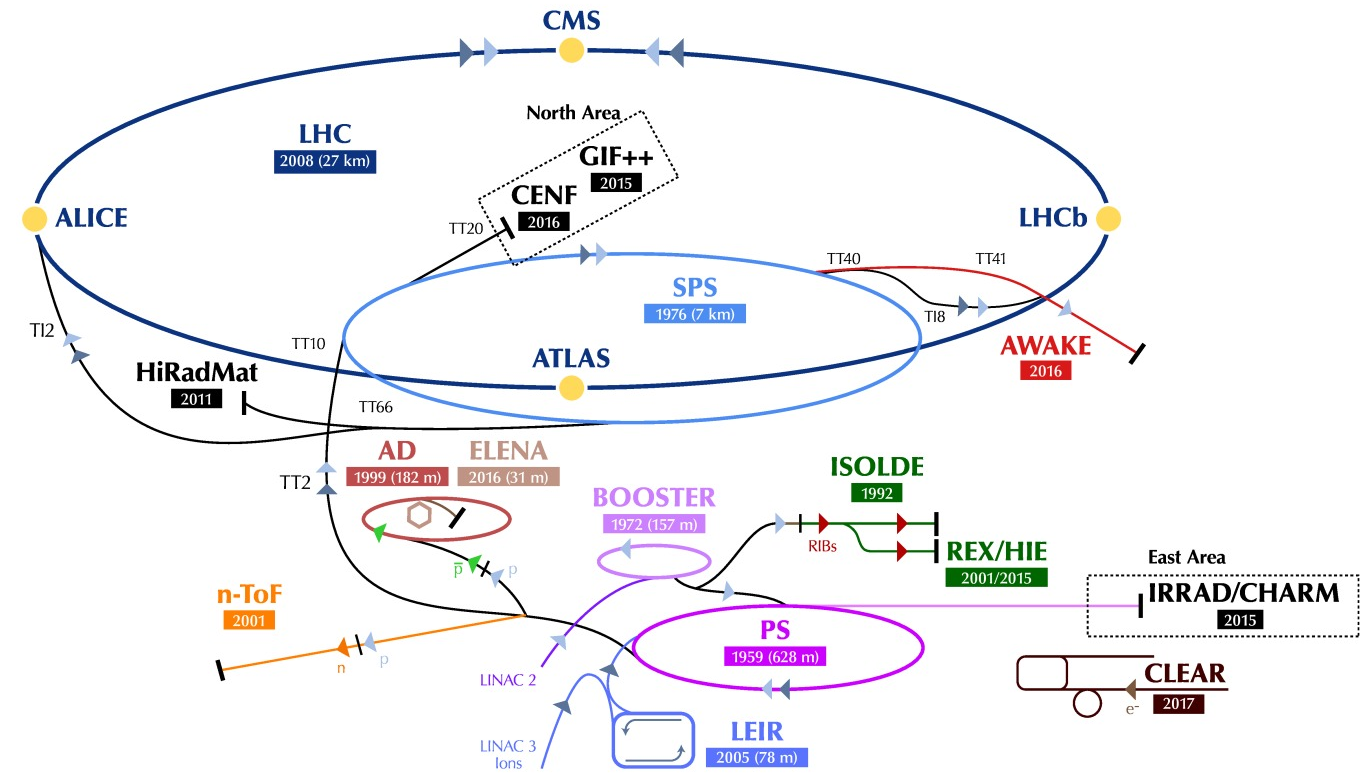
\includegraphics[width=0.8\linewidth]{ALICE/CernComplex_2018.png}        \caption{Complesso dell'intero acceleratore del CERN \\\small{Si vedono  \textcolor{blue}{LHC \textit{Large Hadron Collider}} \textcolor{cyan}{SPS \textit{Super Proton Synchrotron}} \textcolor{purple}{ PS \textit{Proton Synchrotron}} \textcolor{violet}{BOOSTER \textit{ Proton Synchrotron Booster}} LINAC \textit{Linear ACcelerator}} \\{\footnotesize  \textcolor{red}{AD \textit{Antiprotron Decelerator}} \textcolor{green}{ISOLDE \textit{Isotope Separator Online DEvice}}  \textcolor{lightgray}{LEIR \textit{Low Energy Ion Ring}} }}
        \label{fig:CERNcomplex}
    \end{figure}
    
Il fascio di particelle viaggia in un tubo in cui viene fatto l'ultra-vuoto ed è direzionato da dei magneti superconduttivi, che devono essere tenuti alla temperatura di 1.85 $K$.
\\Dal 2008 sono operativi i quattro principali esperimenti di LHC: ALICE, ATLAS, CMS e LHCb. Questi hanno preso dati sia per collisioni protone-protone (\textit{pp}) che per collisioni piombo-piombo (\textit{Pb-Pb}) ed altre. Im questa tesi si utilizzano dati derivanti dall'esperimento ALICE che viene analizzato più nel dettaglio. 



\section{ALICE}

L'acronimo ALICE sta per \textit{"A Large Ion Collider Experiment"} 
    

    
   